\section{Introduction} \label{sec:introduction}
    \IEEEPARstart{R}{espiratory} motion reduces image resolution in \gls{PET} by introducing blurring and mis-alignment artefacts~\cite{Nehmeh2008a}. Unless gated \gls{CT} are available (which themselves increase dose to the patient), to avoid mis-registration due to attenuation mismatches, most existing \gls{MC} methods rely on pair-wise registration of gated \gls{NAC} \gls{PET} volumes~\cite{LungMotionDiaphragmBaiBib}~\cite{Oliveira2014}. This is a challenging problem due to the low contrast and high noise of these volumes. Other \gls{MC} methods can incorporate, directly, both \glsed{MC} and \glss{Mu-Map} estimation into reconstruction, however, these can be computationally expensive~\cite{Bousse2016b}.
    
    Some \glsing{MM} algorithms approach \gls{MC} by fitting a \glss{RCM} on the \glss{DVF} which would deform a \glsed{MCIR} volume \cmmnt{(at the mean respiratory position)} to each input bin and on the \gls{SS} value for that bin. Thus for any given \gls{SS} value the \gls{RCM} returns a \gls{DVF} to warp \cmmnt{either from or to the mean position} to the bin at that \gls{SS} value~\cite{McClelland2013}. A more recent approach uses \glss{DVF} with the corresponding warping operation denoted as $\mathbf{W}(\mathbf{\alpha}_t)$, with $\mathbf{\alpha}_t$ a vector with coefficients at time $t$ and the breathing surrogate signal $\mathbf{s}$:
    
    \begin{equation}
        \forall t \in [[1,n_t]],\quad \alpha_{k,t} := R_{1,k} s_{1,t} + R_{2,k}
    \end{equation}
    
    \noindent where $\alpha_{k,t}$ is the coefficient for node $k$ at time point $t$, and $R_{i,k}$ are the model parameters~\cite{McClelland2017}.
    
    In our previous work we investigated the possibility of using \glsing{MM} for respiratory \gls{MC} where the \gls{RCM} was derived from \gls{NAC} \gls{PET}. We found that \gls{NAC} \gls{TOF} \gls{PET} was suitable to estimate the motion from gated PET data  without inter-respiratory cycle variation~\cite{Whitehead2019ImpactPET}. It is an aim of this work to determine if \gls{NAC} \gls{TOF} data is sufficient to model more complex inter-respiratory cycle motion. In addition, this work extends the method towards attenuation correction with a single \gls{Mu-Map} (from any position) to check if the new method is viable.

\section{Methods} \label{sec:methods}
    \subsection{XCAT Volume Generation} \label{sec:xcat_volume_generation}
        \gls{XCAT}~\cite{Segars2010} was used to generate both $6$ volumes over a single linear \SI{5}{\second} breathing cycle from \gls{XCAT} (henceforth referred to as simple data) and $240$ volumes over a more complex (with inter-respiratory cycle variation) \SI{120}{\second} breathing cycle derived from a respiratory trace captured using an \gls{RPM} (henceforth referred to as complex data). The simple data contained both a volume at full expiration at the beginning of the cycle as well as at the end of the cycle. Both data used max displacement settings for the extent of \gls{AP} and \gls{SI} motion of \SI{1.2}{\centi\metre} and \SI{2.0}{\centi\metre} respectively. Activity concentrations were derived from a static \gls{FDG} patient scan. The \gls{FOV} included the base of the lungs, diaphragm and the top of the liver with a \SI{20}{\milli\metre} diameter spherical lesion placed into the centre of the right lung.
    
    \subsection{PET Acquisition Simulation} \label{sec:pet_acquisition_simulation}
        \gls{PET} acquisitions were simulated (and reconstructed) using \gls{STIR}~\cite{Thielemans2012, Efthimiou2018} through \gls{SIRF}~\cite{ Ovtchinnikov2019CCPPETMRSIRF} to forward project the data using the geometry of a \gls{GE} Discovery 710 with a \gls{TOF} resolution of \SI{375}{\pico\second}. This \gls{TOF} resolution is similar to the \gls{GE} Signa \gls{PET}/\gls{MR}, however, \gls{TOF} mashing is used to reduce computation time resulting in $13$ \gls{TOF} time bins of size \SI{376.5}{\pico\second}. Attenuation was included, in the simulation, using the relevant \glss{Mu-Map} generated by \gls{XCAT}. Scatter and randoms were not taken into account. Multiple noise realisations were generated to simulate an acquisition over \SI{120}{\second}, emulating a standard single bed position acquisition. The simple data was 'pseudo gated', by using noise realisations which (when applied) resulted in as if it had been gated into $6$ bins. The complex data was simulated with realistic noise realisations. A respiratory \gls{SS} was generated for both sets of data using \gls{PCA}~\cite{Thielemans2011}. This was used to gate the data into $10$ bins using displacement gating. For the purpose of the \gls{RCM} fitting, \gls{SS} values were ascertained for the post-gated data by taking an average of the \gls{SS} values of the data in each bin.
    
    \subsection{Non-Attenuation Corrected Image Reconstruction} \label{sec:non-attenuation_corrected_image_reconstruction}
        Data were reconstructed without \gls{AC} using \gls{OSEM} with $2$ full iterations and $24$ subsets~\cite{Hudson1994}. Volumes were post-filtered using a Gaussian blur with a kernel size of \SI{6.4}{\milli\metre} \gls{FWHM}.
    
    \subsection{Motion Model Estimation} \label{sec:motion_model_estimation}
        For each data set \gls{3D} B-spline interpolated \glss{DVF} were used to model spatial deformations. A generalised framework unifying \gls{IR} and respiratory \glss{MM}, NiftyRegResp, was used to estimate \glss{RCM} and \glss{MCIR}~\cite{McClelland2017}. \gls{SSD} was used as the objective function and the second order derivative of the \gls{DVF} was used as a penalty. The \gls{CPG} spacing of the \gls{DVF} and penalty weight were tuned using a grid search.
    
    \subsection{Attenuation Map Warping} \label{sec:attenuation_map_warping}
        A \gls{Mu-Map}, as close to the mean respiratory position as possible, was selected from the \glss{Mu-Map} generated by \gls{XCAT} for both data sets, this \gls{Mu-Map} was then registered to the \gls{MCIR} generated while fitting the \gls{RCM} from~\Fref{sec:motion_model_estimation}. A \gls{NMI} registration was used to accomplish this with parameters selected using a grid search. The \gls{RCM} was then used to generate \gls{DVF} for the \gls{SS} values of each bin, which were then used to warp the \gls{Mu-Map} from the mean respiratory position to each bin.
        
    \subsection{Attenuation Corrected Motion Corrected Image Reconstruction} \label{sec:attenuation_corrected_image_reconstruction}
        Data were re-reconstructed with \gls{AC} using the \glss{Mu-Map} from~\Fref{sec:attenuation_map_warping}. The same reconstruction parameters as in~\Fref{sec:attenuation_corrected_image_reconstruction} were used. This data was then motion corrected again as in~\Fref{sec:motion_model_estimation} to generate a final \gls{AC} \gls{MCIR}.
    
    \subsection{Evaluation} \label{sec:evaluation}
        To evaluate the validity of the \glsing{MM} results, the \gls{COM} of the lesion, over time, was tracked for both \gls{NAC} and \gls{AC} reconstructions of both data sets. This was achieved by warping a volume only including the lesion in the reference position, and then computing its \gls{COM}.
        
        In addition to the reconstructions performed in~\Fref{sec:attenuation_corrected_image_reconstruction} data were also reconstructed by simply summing all gates together and using one \gls{Mu-Map}, positioned as close to the mean respiratory position as possible, for \gls{AC}, this process matches \gls{CCP}. The data from this approach was used for each data set to evaluate the improvement that the new method afforded. The comparisons used included: a visual analysis, a profile over the lesion and \gls{SUV}\textsubscript{max}, \gls{SUV}\textsubscript{median} and \gls{SUV}\textsubscript{peak}. \gls{SUV}\textsubscript{peak} here was defined following \gls{EANM} guidelines~\cite{Boellaard2015FDG2.0}

\section{Results} \label{sec:results}
    \begin{figure}
        \centering
        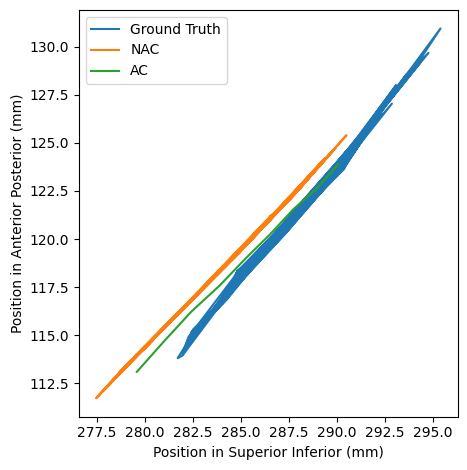
\includegraphics[width=0.5\linewidth]{figures/com.png}
        \captionsetup{singlelinecheck=false, justification=centering}
        \caption{The path of the \gls{COM} of the lesion. Horizontal (respectively vertical) axis corresponds to motion in the \gls{AP} (respectively \gls{SI}) direction over the simple data for (a) and the complex data for (b). Different curves denote \gls{COM} displacement for  ground truth data, the estimated data from the \gls{NAC} based \gls{RCM} and the estimated data from the \gls{AC} based \gls{RCM}.}
        \label{fig:com}
    \end{figure}
    
    \gls{COM} results can be seen in~\Fref{fig:com}, the \gls{COM} of both the \gls{NAC} and \gls{AC} for both the simple and complex data relatively closely matches the ground truth \gls{COM}.
    
    \begin{figure}
        \centering
        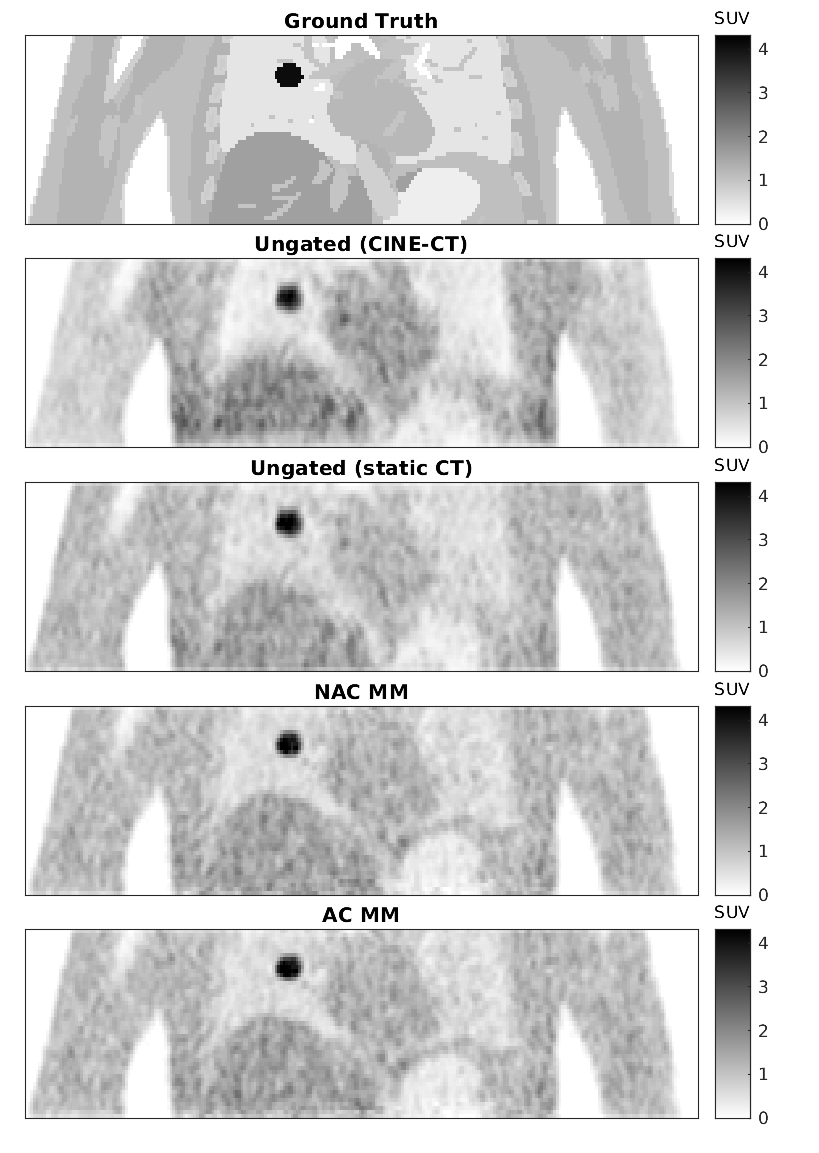
\includegraphics[width=1.0\linewidth]{figures/visual_analysis.png}
        \captionsetup{singlelinecheck=false, justification=centering}
        \caption{First row from left to right: \glsed{CCP} and the new method simple data. Colour map ranges are consistent for all images on this row. Second row: \glsed{CCP} and the new method complex data. Colour map ranges are consistent for all images on this row.}
        \label{fig:visual_analysis}
    \end{figure}
    
    \begin{figure}
        \centering
        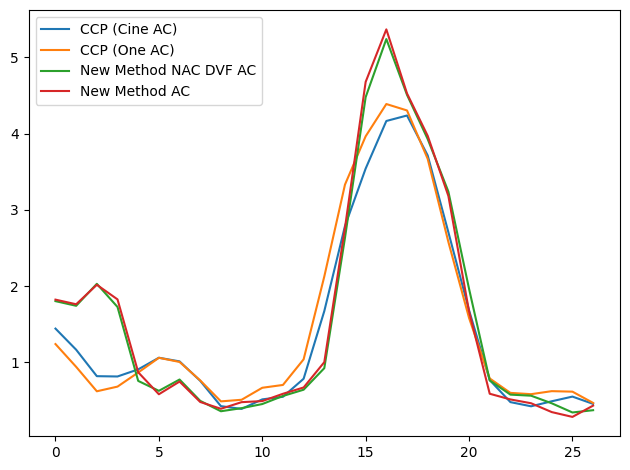
\includegraphics[width=0.5\linewidth]{figures/profile.png}
        \captionsetup{singlelinecheck=false, justification=centering}
        \caption{A profile across the lesion of the simple data for (a) and the complex data for (b). Each sub-figure shows the profile for both the \gls{CCP} as well as for the the new method.}
        \label{fig:profile}
    \end{figure}
    
    \begin{table}
        \centering
        \captionsetup{singlelinecheck=false, justification=centering}
        \caption{Comparison of \gls{SUV}\textsubscript{max}, \gls{SUV}\textsubscript{median} and \gls{SUV}\textsubscript{peak} between the \glsed{CCP} data and the the new method data for both the simple and complex data, plus the difference between \gls{CCP} and the new method \glss{SUV} for each data set.}
        
        \resizebox*{1.0\linewidth}{!}
        {
            \begin{tabular}{||c|ccc||}
                \hline
                \textbf{\gls{SUV}} & \textbf{Max} & \textbf{Median} & \textbf{Peak} \\
                \hline
                \textbf{\gls{CCP} (Cine CT)}            & $4.66$ & $3.05$ & $3.54$ \\
                \textbf{\gls{CCP} (One CT)}             & $4.66$ & $3.05$ & $3.54$ \\
                \textbf{New Method \gls{NAC} \gls{DVF}} & $5.56$ & $3.18$ & $4.07$ \\
                \textbf{New Method \gls{AC} \gls{DVF}}  & $5.43$ & $3.18$ & $4.00$ \\
                \hline
            \end{tabular}
        }
        \label{tab:suv}
    \end{table}
    
     The \gls{CCP} data and the the new method data can be seen in~\Fref{fig:visual_analysis}. When compared visually structures can be seen in the the new method data that cannot be seen in the \gls{CCP} data. For instance, structures at the boundary between the diaphragm and the lung. Additionally, the boundary between the lesion and the lung appears to be sharper and the lesion itself more homogeneous, this can be observed in the profile across the lesion in~\Fref{fig:profile}. \gls{SUV} results can be seen in~\Fref{tab:suv} and consistently show that \glss{SUV} are greater for the new method over \gls{CCP} for both simple and complex data.

\section{Discussion and Conclusions} \label{sec:discussion_and_conclusions}
    \glss{MM} derived from \gls{NAC} \and \gls{AC} volumes for both data containing intra and inter-respiratory cycle motion were found to be relatively robust when comparing \gls{COM}. Results from both a visual analysis and from a comparison of profiles and \glss{SUV} shows that the new method provides volumes freer from blurring and not as susceptible to artefacts when compared to \gls{CCP}.
    
    In the future, research will focus on more complex methods of incorporating, directly, both \glsed{MC} \glss{Mu-Map} and \glsing{MM} into reconstruction.